%!TeX root=../tese.tex
%("dica" para o editor de texto: este arquivo é parte de um documento maior)
% para saber mais: https://tex.stackexchange.com/q/78101/183146

%% ------------------------------------------------------------------------- %%
\chapter{Introdução}
\label{cap:introducao}

\section{Motivação e Objetivos}

Com a crescente ascensão da tecnologia nos dias de hoje o conhecimento sobre
programação tem se tornado cada vez mais importante, não só pelas inúmeras
aplicações que existem, mas também por ser um facilitador, tanto na vida
pessoal quanto na vida profissional.

Devido a esse fato, houve um grande aumento no número de interessados pelo
conhecimento da programação e, consequentemente, o ensino de tal área tem se
difundido cada vez mais. Entretanto, muitos dos interessados por tais técnicas
não dispõem do tempo necessário ou da paciência e concentração para o 
aprendizado tradicional, ou seja, leituras extensas sobre os temas e longas 
sessões práticas para a aplicação das técnicas aprendidas.

Neste momento os jogos ganham força como disseminadores do conhecimento para os 
que buscam o primeiro contato com esta área, pois são
uma forma divertida e rápida de se adquirir experiência básica sobre algo.
Por ser uma forma simples e dinâmica de aprendizado o indíviduo encontra mais
facilidade para encaixar o jogo em sua agenda do que ler um livro teórico sobre
algo. Por isso que o jogo desenvolvido tenta \textit{gamificar} uma plataforma 
de ensino.

Desta forma, visando proporcionar um ambiente facilitador do aprendizado dos
conceitos de programação para indivíduos iniciantes ou com pouca experiência
foi desenvolvido o jogo Phoenix Rising. Além disso a estrutura do código foi
pensada de modo a facilitar a inserção de novas características ao jogo
pelos indivíduos que têm certa experiência em programação, fazendo com que
o projeto desenvolvido sirva para uma grande parte dos interessados em 
aprofundar o conhecimento.


%% ------------------------------------------------------------------------- %%
\section{Organização do Projeto}
\label{sec:consideracoes_preliminares}

O projeto foi desenvolvido utilizando Godot na versão 3.1.1 stable, 
uma \textit{game engine} que facilita a produção de jogos e possui uma linguagem
própria chamada GDScript.
Todo o código do jogo está mantido no GitHub, portanto o projeto é open source,
o que facilita a contribuição pela comunidade.

Como um dos objetivos do projeto é disponibilizar o código fonte para
melhorias serem implementadas, o código e comentários estão em inglês, seguindo
as boas práticas de programação. Vale salientar também que a eficiência não foi
principal ponto do projeto mas sim a legibilidade e a flexibilidade do 
código, portanto em algumas partes preferiu-se utilizar um pouco mais de memória
e/ou processamento, embora tais escolhas não tenham grande impacto na 
jogabilidade.

\chapter{Conceitos Básicos}
\label{cap:Conceitos Básicos}

\section{O Conceito de Árvore}

Para facilitar o entendimento, deve-se entender um pouco sobre o que
é uma árvore no escopo da programação, pois tal conceito aparecerá muitas
vezes neste trabalho, entretanto a definição informal, passando apenas a ideia 
do funcionamento, bastará para entender este projeto.

Árvore refere-se a uma forma de estruturar os dados de um programa,
informalmente pode ser definido como um conjunto de elementos que armazenam 
informações, por sua vez são os chamados nós. Toda árvore possui o elemento 
chamado raiz, que é primeiro nó, de onde a árvore começa, e que possui ligações
para outros elementos denominados filhos, por sua vez também são nós.

\begin{figure}[h]
    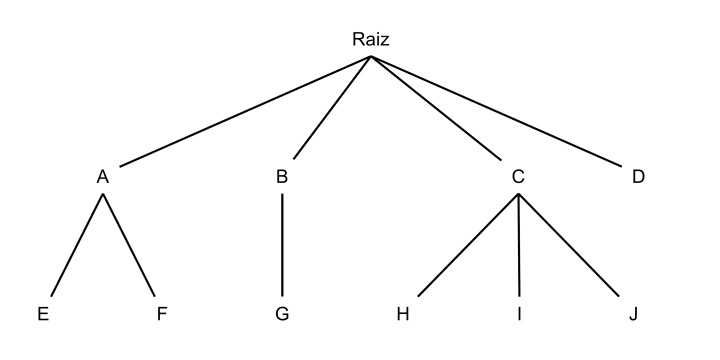
\includegraphics[width=\linewidth]{../figuras/arvore.png}
    \caption{Exemplo de árvore}
\end{figure}   

Perceba que a árvore cresce para baixo, sendo que a raiz dá origem a tudo.
Os nós A, B, C, D são filhos da Raiz. Os nós E, F são filhos do nó A. O nó
D é filho da Raiz e não tem filhos.

Como a estrutura dos projetos criados utilizando a \textit{Godot Engine} é 
baseada em árvores, já é possível entender parte de como o jogo desenvolvido foi 
estruturado. Entretanto ainda é necessário explicar o que é uma 
\textit{Game Engine}.


\section{O que é Game Engine?}

Uma \textit{game engine} é um programa para computador com um conjunto de 
bibliotecas capaz de juntar e construir, em tempo real, todos os elementos de um
jogo.
Ela inclui motor gráfico para renderizar gráficos em 2D ou 3D, motor de física 
para detectar colisões e fazer animações, além de suporte para sons, 
inteligência artificial, gerenciamento de arquivos, programação, entre outros.
Por conta dessas facilidades, a partir do uso de uma \textit{game engine}, é 
possível criar um jogo do zero de maneira mais simples e replicar vários estilos
jogos com mais facilidade.

Escolher a Godot para este projeto teve como motivação o grupo de extensão 
USPGameDev, além do aprendizado ser relativamente simples e de ser um 
\textit{software open source} sob a licença MIT, desenvolvido de forma 
independente pela comunidade.

Como foi estabelecido o conhecimento sobre alguns termos gerais, agora é
possível entender o básico de como funciona a \textit{Godot Engine}.

\section{Entendendo sobre a Godot Engine}

A seguir temos as explicações dos conceitos básicos.

\subsection{Nós}

Nós são blocos de construção fundamentais para a criação de um jogo. Um nó pode
executar uma variedade de funções especializadas.
No entanto, qualquer nó fornecido sempre possui os seguintes atributos:
\begin{itemize}
    \item[$\bullet$]
        Possui um nome.
    \item[$\bullet$]
        Possui propriedades editáveis.
    \item[$\bullet$]
        Ele pode receber um retorno de chamada (\textit{callback}) para 
        processar todos os quadros (\textit{frames}).
    \item[$\bullet$]
        Pode ser estendido (para ter mais funções).
    \item[$\bullet$]
        Pode ser adicionado a outro nó como filho.
\end{itemize}

Perceba que o último atributo é muito importante, pois quando nós tem outros nós
como filhos o conjunto se torna uma árvore, como foi explicado anteriormente.
Em Godot, a capacidade de organizar nós dessa maneira cria uma ferramenta 
poderosa para organizar projetos. Como nós diferentes têm funções diferentes, 
combiná-los permite a criação de funções mais complexas, a partir disso
\textit{Phoenix Rising} foi criado.

\subsection{Cenas}

Uma cena é composta por um grupo de nós organizados hierarquicamente 
(em forma de árvore). Além disso, uma cena:

\begin{itemize}
    \item[$\bullet$]
        Sempre tem um nó raiz.
    \item[$\bullet$]
        Pode ser salvo no disco e carregado de volta.
    \item[$\bullet$]
        Pode ser instanciado (Explicado adiante).
\end{itemize}

Executar um jogo significa executar uma cena. Um projeto pode conter várias 
cenas, mas para o jogo começar, uma delas deve ser selecionada como a cena 
principal.

Basicamente, o editor Godot é um editor de cenas. Possui muitas ferramentas para
editar cenas 2D e 3D, bem como interfaces com o usuário, mas o editor é baseado 
no conceito de edição de uma cena e nos nós que a compõem.

\subsection{Instâncias}

Criar uma única cena e adicionar nós a ela pode funcionar para pequenos 
projetos, mas à medida que o projeto aumenta em tamanho e complexidade, o número
de nós pode se tornar rapidamente incontrolável. Para resolver isso, Godot 
permite que um projeto seja separado em qualquer número de cenas. Isso fornece 
uma ferramenta poderosa que ajuda a organizar os diferentes componentes do seu
jogo.

Em Cenas e nós, você aprendeu que uma cena é uma coleção de nós organizados em 
uma estrutura de árvore, com um único nó como raiz da árvore.
Você pode criar quantas cenas quiser e salvá-las em disco. As cenas salvas dessa
maneira são chamadas de "Cenas compactadas" (\textit{packed scenes}) e têm uma 
extensão de nome de arquivo ".tscn".

A instanciação é muito utilizada em \textit{Phoenix Rising}, portanto esta
parte deve ficar mais clara conforme adentramos nos detalhes da estrutura e
de implementação mais adiante.

\subsection{Árvore de Cena}
\subsection{Sinais}
\subsection{Singleton}
\subsection{GDScripts}

\section{Bibliografia}

\textsc{Referências Bibliográficas} 

https://www.cse.unr.edu/~sushil/class/gas/papers/GameAIp27-lewis.pdf
%https://docs.godotengine.org/en/3.1/getting_started/step_by_step/scenes_and_nodes.html
%https://docs.godotengine.org/en/3.1/getting_started/step_by_step/instancing.html